\documentclass[11pt,a4paper]{report}
\usepackage[utf8]{inputenc}
\usepackage{geometry}
\geometry{margin=1in}
\usepackage{graphicx}
\usepackage{setspace}
\usepackage{titlesec}
\usepackage{array}
\usepackage{booktabs}
\usepackage{caption}
\usepackage{amsmath}
\usepackage{amssymb}
\usepackage{float}
\usepackage{tabularx}
\newcolumntype{Y}{>{\raggedright\arraybackslash}X}
\usepackage{xcolor}
\usepackage{listings}
\usepackage{tikz}
\usetikzlibrary{positioning, arrows.meta, fit, backgrounds}
\usepackage{pgfplots}
\pgfplotsset{compat=1.18}
\usepackage[hidelinks]{hyperref}

% Section numbering depth
\setcounter{secnumdepth}{3}
\renewcommand{\thesection}{\arabic{section}}

% ------------------ Code listing styles ------------------
\definecolor{codebg}{RGB}{248,248,248}
\definecolor{codekw}{RGB}{0,0,160}
\definecolor{codecm}{RGB}{0,110,0}
\definecolor{codestr}{RGB}{160,0,0}
\definecolor{series1}{HTML}{2A78D6}
\lstdefinestyle{base}{
    basicstyle=\ttfamily\scriptsize,
    keywordstyle=\color{codekw}\bfseries,
    commentstyle=\color{codecm}\itshape,
    stringstyle=\color{codestr},
    backgroundcolor=\color{codebg},
    frame=single, rulecolor=\color{gray!60},
    breaklines=true, columns=fullflexible, keepspaces=true,
    showstringspaces=false, tabsize=4,
    numbers=left, numberstyle=\tiny\color{gray}, numbersep=6pt
}
\lstdefinestyle{sql}{
    style=base, language=SQL,
    morekeywords={ROLE,LOGIN,NOLOGIN,PASSWORD,GRANT,REVOKE,USAGE,EXECUTE,POLICY,
                  ENABLE,LEVEL,SECURITY,DEFINER,INVOKER,RETURNS,RETURN,LANGUAGE,
                  DECLARE,BEGIN,END,IF,THEN,RAISE,EXCEPTION,FOUND,STABLE,TRIGGER,
                  BEFORE,AFTER,EACH,ROW,STATEMENT,FUNCTION,PUBLIC,SCHEMA,RETURNING,
                  QUERY,TABLE,BYTEA,JSONB,COALESCE,WITH,SESSION_USER,TRUNCATE}
}
\lstdefinestyle{py}{style=base, language=Python}
\lstset{style=sql}
\captionsetup[lstlisting]{font=small, labelfont=bf}

% ------------------ Diagram styles ------------------
\tikzset{
  actor/.style={draw, rounded corners=3pt, fill=blue!8, font=\scriptsize, align=center,
                minimum width=2.1cm, minimum height=0.75cm},
  comp/.style={draw, fill=green!8, font=\scriptsize, align=center,
               minimum width=2.6cm, minimum height=0.8cm},
  store/.style={draw, fill=orange!12, font=\scriptsize, align=center,
                minimum width=2.4cm, minimum height=0.75cm},
  bad/.style={draw, rounded corners=3pt, fill=red!12, font=\scriptsize, align=center,
              minimum width=2.1cm, minimum height=0.75cm},
  flow/.style={-{Stealth[length=2mm]}, thick},
  atk/.style={-{Stealth[length=2mm]}, thick, red!70!black, dashed},
  zone/.style={draw, dashed, rounded corners=6pt, gray!70!black, inner sep=8pt},
  lbl/.style={font=\scriptsize, align=center}
}

\begin{document}

% ------------------ Cover Page ------------------

\begin{titlepage}
    \centering

    % Ensure 'College Logo RGB.jpg' is in your project folder.
    
\includegraphics[width=5cm]{College Logo RGB.jpg}\\[1cm]

    \vspace{1cm}
    \textbf{\large A Complex Engineering Problem Report on} \\[0.5cm]
    {\LARGE \textbf{Database Security and Privacy Engineering for Sensitive Information Systems}}\\[1.5cm]

    {\Large A9511 - Database Management Systems}\\[1.5cm]

    \textbf{Submitted by}\\ [0.25cm]
    Batch No. 6

    \begin{center}
        \begin{table}[h!]
            \centering
            \setstretch{1.2}
            \begin{tabular}{l l}
                {Madhavarapu Saritha} & {25881A05V7}\\ [2mm]
                {Chepyala Vishal} & {25881A05X9}\\ [2mm]
                {Gundu Srijay Krishna} & {25881A05X0}\\ [2mm]
            \end{tabular}
        \end{table}
    \end{center}

    \vspace{0.5cm}
    \textbf{Course Facilitator}\\ [0.1in]
    {Dr. Reddy Saisindhutheja}\\
    Associate Professor\\[2.5cm]

    {\large\textbf{Department of Computer Science and Engineering}}\\[0.5cm]
    {\large\textbf{Vardhaman College of Engineering, Hyderabad}}\\[0.5cm]
    {\large \textbf{November 2026}}

\end{titlepage}

% ------------------ Contents ------------------

\tableofcontents
\newpage

% ------------------ Section 1: Problem Definition ------------------

\section{Problem Definition and Context}

\subsection{Sensitive Data in a Student Information System}
A college Student Information System (SIS) holds some of the most sensitive data an institution owns. This includes identity numbers (Aadhaar), contact details and dates of birth, academic marks that decide careers, and fee-payment records. The same database is used every day by very different people: registrar staff, faculty, students, the accounts section and auditors. A single weakness, such as a vulnerable web form, an over-privileged account or an unencrypted backup, can expose the records of thousands of students at once.

\textbf{Problem Statement:} A student/customer database must satisfy confidentiality, integrity and data-protection regulations. Design role-based access, encryption, auditing and SQL injection defences, and analyse the conflict between security controls and usability or performance.

\textbf{What has to be done:}
\begin{enumerate}
    \item Build a threat model listing assets, threats and attackers for the database.
    \item Implement roles, least-privilege grants, views and row-level security.
    \item Demonstrate an SQL injection on a vulnerable query and fix it with parameterized queries.
    \item Encrypt sensitive columns and enable audit logging.
    \item Measure the performance overhead and discuss its impact on usability.
\end{enumerate}

\textbf{Regulatory context.} India's \emph{Digital Personal Data Protection (DPDP) Act, 2023} requires every data fiduciary to protect personal data by taking ``reasonable security safeguards to prevent personal data breach'' (Section 8(5)), and failure can attract penalties of up to Rs.\,250 crore. The DPDP Rules, 2025 name encryption, masking, access control and access logs as examples of such safeguards. UIDAI additionally requires Aadhaar numbers to be stored only in encrypted form in a secure ``Aadhaar Data Vault''. The design in this report maps directly to these obligations.

All controls were implemented and tested on \textbf{PostgreSQL 16.14} with the \texttt{pgcrypto} extension. The application-side demonstration uses Python 3 with \texttt{psycopg2}. Every result quoted below was produced by running the scripts supplied with this report.

\subsection{Why This Is a Complex Engineering Problem}
\begin{table}[H]
    \centering
    \caption{Characteristics of a Complex Engineering Problem (WP1--WP7) addressed in this work}
    \small
    \setstretch{1.15}
    \begin{tabularx}{\textwidth}{|l|Y|}
        \hline
        \textbf{Attribute} & \textbf{How it appears in this problem} \\ \hline
        WP1 Depth of knowledge & Requires DBMS internals (RLS, view security, triggers), applied cryptography (AES, HMAC, key derivation) and secure coding. \\ \hline
        WP2 Conflicting requirements & Stronger security (encryption, auditing, masking) costs speed and convenience; the right balance has to be measured, not assumed. \\ \hline
        WP3 Depth of analysis & Threat modelling with risk scoring, attack simulation and quantitative performance measurement. \\ \hline
        WP4 Infrequently encountered issues & Searching encrypted data (blind index), definer- vs.\ invoker-rights views, and RLS policy evaluation cost. \\ \hline
        WP5 Extent of applicable codes & DPDP Act 2023, UIDAI Aadhaar Data Vault requirement, OWASP and NIST guidance. \\ \hline
        WP6 Stakeholder involvement & Students, faculty, registrar, accounts, auditors and regulators each need different access. \\ \hline
        WP7 Interdependence & Roles, RLS, encryption, views and audit triggers interact; a change in one affects the others. \\ \hline
    \end{tabularx}
\end{table}

\subsection{Relevance to Sustainable Development Goals (SDGs)}
\begin{itemize}
    \item \textbf{SDG 16 (Peace, Justice and Strong Institutions):} Protecting personal data safeguards the fundamental right to privacy (Target 16.10), and tamper-proof audit trails make institutions accountable (Target 16.6).
    \item \textbf{SDG 9 (Industry, Innovation and Infrastructure):} Secure-by-design databases are part of resilient and trustworthy digital infrastructure.
    \item \textbf{SDG 4 (Quality Education):} Students and parents can trust digital academic systems only when marks cannot be tampered with and personal data cannot leak.
\end{itemize}

% ------------------ Section 2: Problem Analysis ------------------

\section{Problem Analysis and Solution Development}

\subsection{Characterization of the Problem}
The system stores four kinds of data with very different sensitivity (Table~\ref{tab:classify}). A naive design gives the application one powerful database account and leaves every check to the application code. That design fails in three ways: one bug (for example, SQL injection) exposes everything; insiders can see far more than their job needs; and nobody can prove who changed a mark or viewed an Aadhaar number. The goal is \emph{defence in depth}, so that the database itself enforces confidentiality and integrity even when the application layer fails.

\begin{table}[H]
    \centering
    \caption{Data classification of the SIS}
    \label{tab:classify}
    \small
    \setstretch{1.15}
    \begin{tabularx}{\textwidth}{|l|Y|l|l|}
        \hline
        \textbf{Data} & \textbf{Columns} & \textbf{Class} & \textbf{Main concern} \\ \hline
        Identity numbers & \texttt{aadhaar\_enc}, \texttt{phone\_enc} & Restricted & Confidentiality \\ \hline
        Personal profile & \texttt{full\_name}, \texttt{email}, \texttt{dob} & Confidential & Confidentiality \\ \hline
        Academic records & \texttt{marks.internal}, \texttt{marks.external} & Confidential & Integrity \\ \hline
        Financial records & \texttt{fee\_payment.*} & Confidential & Integrity \\ \hline
        Encryption keys & \texttt{vault.data\_key} & Restricted & Confidentiality \\ \hline
        Audit trail & \texttt{audit.log} & Internal & Integrity, non-repudiation \\ \hline
        Reference data & \texttt{department}, \texttt{course} & Internal & Availability \\ \hline
    \end{tabularx}
\end{table}

\subsection{Engineering Knowledge Applied}
\begin{itemize}
    \item \textbf{Security Principles:} Least privilege, separation of duties, complete mediation and defence in depth (Saltzer and Schroeder).
    \item \textbf{Threat Modelling:} STRIDE classification with likelihood $\times$ impact risk scoring.
    \item \textbf{Access Control:} Role-Based Access Control (RBAC), column-level privileges, PostgreSQL Row-Level Security (RLS), security-barrier and security-invoker views, \texttt{SECURITY DEFINER} functions.
    \item \textbf{Applied Cryptography:} AES-256 (OpenPGP symmetric encryption via \texttt{pgcrypto}), HMAC-SHA256 blind indexing, salted key derivation, SCRAM-SHA-256 authentication and TLS.
    \item \textbf{Secure Coding:} Parameterized queries and allow-list input validation against SQL injection (OWASP).
    \item \textbf{Performance Engineering:} Controlled benchmarking, query-plan analysis and overhead quantification.
\end{itemize}

\subsection{Threat Model}
\label{sec:threat}
\subsubsection{System Context and Trust Boundaries}
Figure~\ref{fig:dfd} shows who talks to the database and where trust boundaries lie. Red dashed arrows are attack paths that the controls in this report must block.

\begin{figure}[!htbp]
\centering
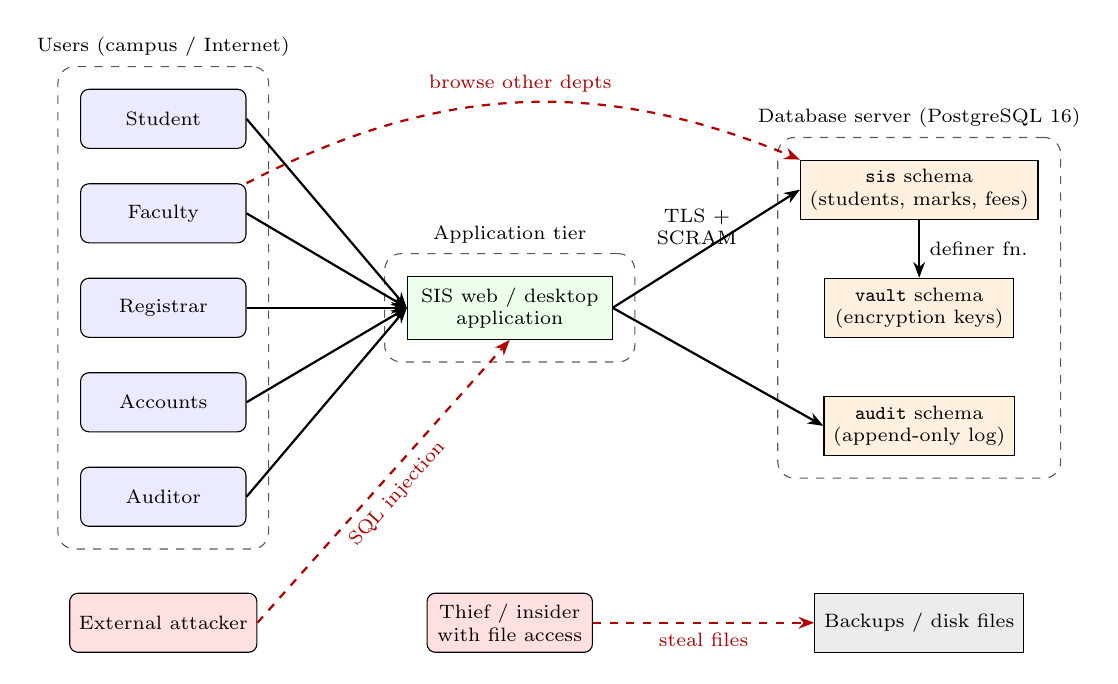
\begin{tikzpicture}[node distance=0.5cm and 1.0cm]
  % users
  \node[actor] (stu) at (0,2.4) {Student};
  \node[actor] (fac) at (0,1.2) {Faculty};
  \node[actor] (reg) at (0,0.0) {Registrar};
  \node[actor] (acc) at (0,-1.2) {Accounts};
  \node[actor] (aud) at (0,-2.4) {Auditor};
  \node[bad]   (ext) at (0,-4.0) {External attacker};
  % app
  \node[comp] (app) at (4.4,0) {SIS web / desktop\\application};
  % db
  \node[store] (sis) at (9.6,1.5) {\texttt{sis} schema\\(students, marks, fees)};
  \node[store] (vlt) at (9.6,0.0) {\texttt{vault} schema\\(encryption keys)};
  \node[store] (aul) at (9.6,-1.5) {\texttt{audit} schema\\(append-only log)};
  \node[store, fill=gray!15] (bak) at (9.6,-4.0) {Backups / disk files};
  \node[bad] (ins) at (4.4,-4.0) {Thief / insider\\with file access};
  % zones
  \begin{scope}[on background layer]
    \node[zone, fit=(stu)(aud), label={[lbl]above:Users (campus / Internet)}] {};
    \node[zone, fit=(app), label={[lbl]above:Application tier}] {};
    \node[zone, fit=(sis)(aul), label={[lbl]above:Database server (PostgreSQL 16)}] {};
  \end{scope}
  % flows
  \foreach \x in {stu,fac,reg,acc,aud} \draw[flow] (\x.east) -- (app.west);
  \draw[flow] (app.east) -- node[lbl,above,pos=0.45]{TLS +\\SCRAM} (sis.west);
  \draw[flow] (app.east) -- (aul.west);
  \draw[flow] (sis) -- node[lbl,right]{definer fn.} (vlt);
  % attacks
  \draw[atk] (ext.east) -- node[lbl,below,sloped]{SQL injection} (app.south);
  \draw[atk] (ins.east) -- node[lbl,below]{steal files} (bak.west);
  \draw[atk] (fac.north east) to[bend left=25] node[lbl,above]{browse other depts} (sis.north west);
\end{tikzpicture}
\caption{Data-flow diagram with trust boundaries (dashed boxes) and attack paths (red)}
\label{fig:dfd}
\end{figure}

\subsubsection{Assets and Attackers}
\begin{table}[H]
    \centering
    \caption{Threat agents (attackers)}
    \small
    \setstretch{1.15}
    \begin{tabularx}{\textwidth}{|>{\raggedright\arraybackslash}p{3.7cm}|Y|>{\raggedright\arraybackslash}p{3.6cm}|}
        \hline
        \textbf{Attacker} & \textbf{Motivation and capability} & \textbf{Typical target} \\ \hline
        External attacker & Data theft for fraud or resale; uses automated SQL injection tools & All PII, encryption keys \\ \hline
        Curious/malicious student & Change own marks, view classmates' data; has a valid login & Marks, other students' records \\ \hline
        Curious faculty member & Browse students of other departments; has a valid login & Student profiles \\ \hline
        Privileged insider (registrar, DBA) & Misuse legitimate access to PII and then hide traces & Aadhaar/phone, audit log \\ \hline
        Physical/backup thief & Copies disk images or backup files & Data at rest \\ \hline
        Network eavesdropper & Sniffs traffic between application and database & Credentials, query results \\ \hline
    \end{tabularx}
\end{table}

\subsubsection{STRIDE Threat Analysis and Risk Scoring}
Each threat is rated for likelihood $L$ and impact $I$ on a 1--5 scale. The risk score is
$$R = L \times I, \qquad \text{High if } R \ge 15,\quad \text{Medium if } 8 \le R < 15,\quad \text{Low if } R < 8.$$

\begin{table}[H]
    \centering
    \caption{STRIDE threats, risk before controls, and the control that mitigates each one}
    \label{tab:stride}
    \footnotesize
    \setstretch{1.15}
    \begin{tabularx}{\textwidth}{|c|Y|c|c|c|c|Y|}
        \hline
        \textbf{\#} & \textbf{Threat} & \textbf{STRIDE} & \textbf{L} & \textbf{I} & \textbf{R} & \textbf{Control (section)} \\ \hline
        T1 & SQL injection through the result portal & T, I, E & 4 & 5 & \textbf{20} & Parameterized queries, input validation, least privilege (\ref{sec:sqli}) \\ \hline
        T2 & Student modifies own marks & T & 3 & 5 & \textbf{15} & No \texttt{UPDATE} grant, RLS, audit (\ref{sec:rbac}, \ref{sec:audit}) \\ \hline
        T3 & Faculty views students of other departments & I & 4 & 3 & 12 & RLS + column privileges (\ref{sec:rbac}) \\ \hline
        T4 & Registrar misuses Aadhaar/phone data & I, R & 3 & 4 & 12 & Masking, break-glass reveal with reason and daily limit (\ref{sec:enc}) \\ \hline
        T5 & Stolen password or brute-force login & S & 3 & 4 & 12 & Per-user logins, SCRAM-SHA-256, strong passwords (\ref{sec:enc}) \\ \hline
        T6 & Theft of database files or backups & I & 2 & 5 & 10 & Column encryption (AES-256), keys isolated (\ref{sec:enc}) \\ \hline
        T7 & Faculty edits marks of a course they do not teach & T & 2 & 4 & 8 & RLS \texttt{WITH CHECK} (\ref{sec:rbac}) \\ \hline
        T8 & Insider deletes audit records to hide misuse & R & 2 & 4 & 8 & Append-only log, separate auditor role (\ref{sec:audit}) \\ \hline
        T9 & Eavesdropping between application and database & I & 2 & 4 & 8 & TLS (\texttt{hostssl}) (\ref{sec:enc}) \\ \hline
        T10 & Expensive queries exhaust the server & D & 2 & 3 & 6 & \texttt{statement\_timeout}, per-role connection limits \\ \hline
    \end{tabularx}
\end{table}
\noindent\textit{STRIDE: S = Spoofing, T = Tampering, R = Repudiation, I = Information disclosure, D = Denial of service, E = Elevation of privilege.}

\subsection{Roles, Least-Privilege Grants, Views and Row-Level Security}
\label{sec:rbac}
\subsubsection{Role Design}
Privileges are given to five \emph{group roles} that match job functions. Each human gets a personal \emph{login role} that inherits exactly one group role. All objects belong to \texttt{sis\_owner}, a role that \emph{cannot log in}. Default privileges for \texttt{PUBLIC} are revoked from the database, the schemas and every function.

\begin{lstlisting}[caption={Role hierarchy (from \texttt{01\_roles.sql})}]
CREATE ROLE sis_owner NOLOGIN;            -- owns every object, nobody logs in as it
CREATE ROLE r_admin_office NOLOGIN;       -- registrar / exam cell
CREATE ROLE r_faculty      NOLOGIN;       -- teaching staff
CREATE ROLE r_student      NOLOGIN;       -- students (self-service)
CREATE ROLE r_accounts     NOLOGIN;       -- fee section
CREATE ROLE r_auditor      NOLOGIN;       -- internal audit / DPO

CREATE ROLE fac_kumar      LOGIN PASSWORD '...' IN ROLE r_faculty;   -- one per person
CREATE ROLE stu_25881a0501 LOGIN PASSWORD '...' IN ROLE r_student;

REVOKE ALL ON DATABASE sis_db FROM PUBLIC;
REVOKE CREATE ON SCHEMA public FROM PUBLIC;
\end{lstlisting}

\begin{table}[H]
    \centering
    \caption{Privilege matrix (rows visible are further limited by RLS)}
    \label{tab:matrix}
    \scriptsize
    \setlength{\tabcolsep}{3pt}
    \setstretch{1.15}
    \begin{tabularx}{\textwidth}{|l|Y|Y|Y|Y|Y|}
        \hline
        \textbf{Object} & \textbf{r\_admin\_office} & \textbf{r\_faculty} & \textbf{r\_student} & \textbf{r\_accounts} & \textbf{r\_auditor} \\ \hline
        \texttt{student} & SELECT all; UPDATE name, email, dept; INSERT only via \texttt{register\_}\allowbreak\texttt{student()} & SELECT 5 non-PII columns, own department & SELECT 6 columns, own row & SELECT 4 columns & -- \\ \hline
        \texttt{marks} & SELECT, INSERT, UPDATE & SELECT, UPDATE (internal, external), own courses & SELECT own & -- & -- \\ \hline
        \texttt{fee\_payment} & SELECT & -- & SELECT own & SELECT, INSERT & -- \\ \hline
        \texttt{v\_student\_masked} & SELECT & -- & -- & SELECT & -- \\ \hline
        \texttt{v\_marks\_sheet} & SELECT & SELECT & SELECT & -- & -- \\ \hline
        \texttt{reveal\_pii()} & EXECUTE & -- & -- & -- & -- \\ \hline
        \texttt{audit.log} & -- & -- & -- & -- & SELECT \\ \hline
        \texttt{vault.*} & -- & -- & -- & -- & -- \\ \hline
    \end{tabularx}
\end{table}

\begin{lstlisting}[caption={Column-level least-privilege grants (from \texttt{04\_access\_control.sql})}]
GRANT SELECT ON sis.student TO r_admin_office;
GRANT UPDATE (full_name, email, dept_id) ON sis.student TO r_admin_office;
GRANT SELECT (student_id, roll_no, full_name, email, dept_id)      ON sis.student TO r_faculty;
GRANT SELECT (student_id, roll_no, full_name, email, dept_id, dob) ON sis.student TO r_student;
GRANT SELECT (student_id, roll_no, full_name, dept_id)             ON sis.student TO r_accounts;

GRANT SELECT, INSERT, UPDATE ON sis.marks TO r_admin_office;
GRANT SELECT, UPDATE (internal, external) ON sis.marks TO r_faculty;
GRANT SELECT ON sis.marks TO r_student;

GRANT SELECT, INSERT ON sis.fee_payment TO r_accounts;
GRANT SELECT ON sis.fee_payment TO r_admin_office, r_student;
\end{lstlisting}

\subsubsection{Row-Level Security Policies}
Grants decide \emph{which tables and columns} a role may touch; RLS decides \emph{which rows}. Small \texttt{SECURITY DEFINER} helper functions map the login (\texttt{session\_user}) to a faculty or student identity. Wrapping the helper as \texttt{(SELECT fn())} makes PostgreSQL evaluate it once per query instead of once per row; Section~\ref{sec:perf} measures why this matters.

\begin{lstlisting}[caption={Identity helper and RLS policies}]
CREATE FUNCTION sis.my_dept() RETURNS SMALLINT
LANGUAGE sql STABLE SECURITY DEFINER SET search_path = pg_catalog, sis AS $$
    SELECT dept_id FROM sis.faculty WHERE db_user = session_user;
$$;

ALTER TABLE sis.student ENABLE ROW LEVEL SECURITY;
CREATE POLICY student_admin    ON sis.student FOR ALL    TO r_admin_office
       USING (true) WITH CHECK (true);
CREATE POLICY student_faculty  ON sis.student FOR SELECT TO r_faculty
       USING (dept_id = (SELECT sis.my_dept()));
CREATE POLICY student_self     ON sis.student FOR SELECT TO r_student
       USING (student_id = (SELECT sis.my_student_id()));
CREATE POLICY student_accounts ON sis.student FOR SELECT TO r_accounts
       USING (true);

ALTER TABLE sis.marks ENABLE ROW LEVEL SECURITY;
CREATE POLICY marks_faculty_edit ON sis.marks FOR UPDATE TO r_faculty
       USING      (course_id IN (SELECT course_id FROM sis.course
                                  WHERE faculty_id = (SELECT sis.my_faculty_id())))
       WITH CHECK (course_id IN (SELECT course_id FROM sis.course
                                  WHERE faculty_id = (SELECT sis.my_faculty_id())));
CREATE POLICY marks_self ON sis.marks FOR SELECT TO r_student
       USING (student_id = (SELECT sis.my_student_id()));
-- (similar policies for marks_admin, marks_faculty_read and fee_payment)
\end{lstlisting}

\subsubsection{Views: Definer Rights vs.\ Invoker Rights}
PostgreSQL views normally run with the \emph{owner's} privileges. This is used deliberately for one view and avoided for the other:
\begin{itemize}
    \item \texttt{v\_student\_masked} runs with owner rights, so it can read the ciphertext columns. It decrypts them only through \texttt{sis.mask()}, which returns just the last four characters. \texttt{security\_barrier} stops a caller from using a leaky function in a \texttt{WHERE} clause to see rows before masking.
    \item \texttt{v\_marks\_sheet} is declared \texttt{security\_invoker = true}, so the caller's own grants and RLS policies on \texttt{student} and \texttt{marks} decide what each user sees through the same view.
\end{itemize}

\begin{lstlisting}[caption={Masking view and invoker-rights view}]
CREATE FUNCTION sis.mask(p_cipher BYTEA, p_prefix TEXT) RETURNS TEXT
LANGUAGE sql STABLE SECURITY DEFINER SET search_path = pg_catalog AS $$
    SELECT p_prefix || right(vault.dec(p_cipher), 4);
$$;

CREATE VIEW sis.v_student_masked WITH (security_barrier = true) AS
SELECT s.roll_no, s.full_name, d.dept_code,
       sis.mask(s.phone_enc,   'XXXXXX')      AS phone_masked,
       sis.mask(s.aadhaar_enc, 'XXXX-XXXX-')  AS aadhaar_masked
FROM sis.student s JOIN sis.department d ON d.dept_id = s.dept_id;
GRANT SELECT ON sis.v_student_masked TO r_accounts, r_admin_office;

CREATE VIEW sis.v_marks_sheet WITH (security_invoker = true) AS
SELECT s.roll_no, s.full_name, c.course_code,
       m.internal, m.external, m.internal + m.external AS total
FROM sis.marks m
JOIN sis.student s ON s.student_id = m.student_id
JOIN sis.course  c ON c.course_id  = m.course_id;
GRANT SELECT ON sis.v_marks_sheet TO r_admin_office, r_faculty, r_student;
\end{lstlisting}

\subsubsection{Verification}
The script \texttt{06\_verify.sql} logs in as each user (\texttt{SET SESSION AUTHORIZATION}) and tries both allowed and forbidden actions. The sample data has 6 students (3 CSE, 2 ECE, 1 MECH).

\begin{table}[H]
    \centering
    \caption{Access-control test results}
    \label{tab:verify}
    \footnotesize
    \setstretch{1.15}
    \begin{tabularx}{\textwidth}{|c|l|Y|Y|c|}
        \hline
        \textbf{\#} & \textbf{User} & \textbf{Action} & \textbf{Observed result} & \textbf{Pass} \\ \hline
        T2 & fac\_kumar (CSE) & \texttt{SELECT ... FROM sis.student} & 3 rows, all CSE & \checkmark \\ \hline
        T3 & fac\_kumar & \texttt{SELECT phone\_enc FROM sis.student} & \texttt{permission denied for table student} & \checkmark \\ \hline
        T4 & fac\_kumar & \texttt{SELECT * FROM v\_marks\_sheet} & 6 rows, only CS301/CS302 & \checkmark \\ \hline
        T5 & fac\_kumar & \texttt{UPDATE} a CS301 mark / an EC301 mark & \texttt{UPDATE 1} / \texttt{UPDATE 0} (row invisible) & \checkmark \\ \hline
        T6 & fac\_rao (ECE) & \texttt{SELECT ... FROM sis.student} & 2 rows, both ECE & \checkmark \\ \hline
        T7 & stu\_25881a0501 & Read student, marks sheet, fees & Only own row, own 2 marks, own 1 payment & \checkmark \\ \hline
        T8 & stu\_25881a0501 & \texttt{UPDATE sis.marks SET external = 60} & \texttt{permission denied for table marks} & \checkmark \\ \hline
        T9 & acc\_meena & \texttt{SELECT * FROM v\_student\_masked} & \texttt{XXXXXX0001}, \texttt{XXXX-XXXX-0001}, \dots & \checkmark \\ \hline
        T9 & acc\_meena & Read \texttt{marks}; read \texttt{vault.data\_key} & \texttt{permission denied} (both) & \checkmark \\ \hline
        T10 & admin\_ravi & \texttt{reveal\_pii('25881A0502', 'x')} & \texttt{A justification of at least 10 characters is required} & \checkmark \\ \hline
        T10 & admin\_ravi & \texttt{DELETE FROM audit.log} & \texttt{permission denied for schema audit} & \checkmark \\ \hline
        T12 & sis\_owner & \texttt{UPDATE} / \texttt{TRUNCATE audit.log} & \texttt{audit.log is append-only (... blocked)} & \checkmark \\ \hline
    \end{tabularx}
\end{table}

\subsection{SQL Injection: Attack Demonstration and Fix}
\label{sec:sqli}
\subsubsection{The Vulnerable Query}
A typical ``check your result'' page takes a roll number from the user and pastes it into the SQL text:

\begin{lstlisting}[style=py, caption={Vulnerable lookup (from \texttt{app/injection\_demo.py})}]
def result_lookup_vulnerable(conn, roll_no):
    sql = ("SELECT roll_no, full_name, course_code, total "
           "FROM sis.v_marks_sheet WHERE roll_no = '" + roll_no + "'")
    with conn.cursor() as cur:
        cur.execute(sql)
        return cur.fetchall() if cur.description else []
\end{lstlisting}

Because the input becomes part of the SQL text, an attacker can close the string literal and append their own SQL. Three classic payloads were tested (Table~\ref{tab:payloads}).

\begin{table}[H]
    \centering
    \caption{Injection payloads}
    \label{tab:payloads}
    \footnotesize
    \setstretch{1.15}
    \begin{tabularx}{\textwidth}{|l|Y|Y|}
        \hline
        \textbf{Type} & \textbf{Input typed into the roll-number box} & \textbf{Goal} \\ \hline
        Tautology & \texttt{' OR '1'='1} & Make the \texttt{WHERE} clause always true and dump every row \\ \hline
        UNION & \texttt{' UNION SELECT purpose, encode(key\_bytes,'hex'), NULL, NULL FROM vault.data\_key -{}-} & Read another table: the encryption keys \\ \hline
        Stacked query & \texttt{'; UPDATE sis.marks SET external = 60; -{}-} & Run a second statement that changes data \\ \hline
    \end{tabularx}
\end{table}

\subsubsection{Results}
\textbf{Part A: vulnerable code with an over-privileged account.} Many applications connect as the table owner. Simulating this with \texttt{legacy\_app} (a member of \texttt{sis\_owner}), every attack succeeded:
\begin{itemize}
    \item Tautology returned \textbf{all 9} marks rows of all students instead of the 2 rows of one student.
    \item The UNION payload returned the \textbf{encryption and HMAC keys}, which makes column encryption useless:\\
    {\scriptsize\texttt{('ENC', '29aec9e2c0ffbbacd06377350675\dots f1722c34', None, None)}}
    \item The stacked query changed the external mark of \textbf{every} student to 60 (\texttt{9 of 9} rows tampered).
\end{itemize}

\textbf{Part B: the same vulnerable code with a least-privilege account.} Connected as student \texttt{stu\_25881a0501}, the injection still ``works'' syntactically, but the database limits the damage:
\begin{itemize}
    \item Tautology returned only the student's \textbf{own 2 rows}, because RLS filters the rows regardless of the \texttt{WHERE} clause.
    \item UNION on the keys: \texttt{permission denied for schema vault}.
    \item Stacked \texttt{UPDATE}: \texttt{permission denied for table marks}.
\end{itemize}

\textbf{Part C: the fix.} The input is first checked against the roll-number format, then passed as a \emph{bound parameter}, so the driver sends it strictly as a string value and never as SQL code:

\begin{lstlisting}[style=py, caption={Fixed lookup with validation and a parameterized query}]
ROLL_NO = re.compile(r"[0-9]{2}881A[0-9]{2}[0-9A-Z]{2}")

def result_lookup_safe(conn, roll_no):
    if not ROLL_NO.fullmatch(roll_no):
        raise ValueError("invalid roll number format")
    with conn.cursor() as cur:
        cur.execute("SELECT roll_no, full_name, course_code, total "
                    "FROM sis.v_marks_sheet WHERE roll_no = %s", (roll_no,))
        return cur.fetchall()
\end{lstlisting}

Even with the over-privileged \texttt{legacy\_app} account, all three payloads were rejected by validation. With validation removed, the parameterized query searched for the literal string \texttt{' OR '1'='1}, found \textbf{0 rows} and changed nothing. The SQL actually sent to the server shows that the quotes were escaped:
\begin{center}
\texttt{... WHERE roll\_no = '{}'{}' OR '{}'1'{}'='{}'1'}
\end{center}

\textbf{Lesson.} Parameterized queries remove the vulnerability; least privilege and RLS limit the damage if a vulnerability is ever missed. Both layers are needed.

\subsection{Encryption of Sensitive Columns}
\label{sec:enc}
\subsubsection{Design}
\begin{itemize}
    \item \textbf{Algorithm:} \texttt{pgp\_sym\_encrypt} (OpenPGP, RFC 4880) with \textbf{AES-256}. Each value gets a random salt and session key, so two students with the same phone number have different ciphertexts. This prevents frequency analysis, and a built-in integrity check detects tampered ciphertext.
    \item \textbf{Key derivation choice:} the key is 256 random bits, not a human password. Password stretching (\texttt{s2k-mode=3}) therefore adds cost but no security, and \texttt{s2k-mode=1} (salted, single pass) is used. Section~\ref{sec:perf} shows this makes encryption \textbf{26$\times$ faster}.
    \item \textbf{Key isolation:} keys live in \texttt{vault.data\_key}. No role except the non-login owner has \texttt{USAGE} on the \texttt{vault} schema; keys are reachable only through \texttt{SECURITY DEFINER} functions whose \texttt{EXECUTE} right has been revoked from \texttt{PUBLIC}.
    \item \textbf{Searching encrypted data:} an encrypted column cannot be searched with \texttt{=}, because each encryption differs. A \textbf{blind index}, $\text{HMAC-SHA256}(k_2, \text{aadhaar})$, stored in a \texttt{UNIQUE} column, allows exact-match lookup and duplicate detection without revealing the number.
    \item \textbf{Data in transit:} \texttt{ssl = on} in \texttt{postgresql.conf}, \texttt{hostssl ... scram-sha-256} lines in \texttt{pg\_hba.conf}, and \texttt{password\_encryption = scram-sha-256}.
\end{itemize}

\begin{lstlisting}[caption={Key vault and encryption functions (from \texttt{02\_schema.sql})}]
CREATE TABLE vault.data_key (
    purpose    VARCHAR(10) PRIMARY KEY CHECK (purpose IN ('ENC','HMAC')),
    key_bytes  BYTEA       NOT NULL CHECK (length(key_bytes) = 32),
    created_at TIMESTAMPTZ NOT NULL DEFAULT now()
);
INSERT INTO vault.data_key (purpose, key_bytes) VALUES
    ('ENC', gen_random_bytes(32)), ('HMAC', gen_random_bytes(32));

CREATE FUNCTION vault.enc(p_plain TEXT) RETURNS BYTEA
LANGUAGE sql STABLE SECURITY DEFINER SET search_path = pg_catalog, public AS $$
    SELECT pgp_sym_encrypt(p_plain, encode(key_bytes, 'hex'),
                           'cipher-algo=aes256, s2k-mode=1')
    FROM vault.data_key WHERE purpose = 'ENC';
$$;

CREATE FUNCTION vault.blind_index(p_plain TEXT) RETURNS BYTEA
LANGUAGE sql STABLE SECURITY DEFINER SET search_path = pg_catalog, public AS $$
    SELECT hmac(convert_to(p_plain, 'UTF8'), key_bytes, 'sha256')
    FROM vault.data_key WHERE purpose = 'HMAC';
$$;
REVOKE ALL ON ALL FUNCTIONS IN SCHEMA vault FROM PUBLIC;
REVOKE ALL ON SCHEMA vault FROM PUBLIC;

-- The only way to create a student: validates and encrypts the PII
CREATE FUNCTION sis.register_student(p_roll TEXT, p_name TEXT, p_email TEXT,
       p_dept SMALLINT, p_dob DATE, p_phone TEXT, p_aadhaar TEXT,
       p_db_user NAME DEFAULT NULL) RETURNS INT
LANGUAGE plpgsql SECURITY DEFINER SET search_path = pg_catalog, sis AS $$
DECLARE v_id INT;
BEGIN
    IF p_phone   !~ '^[6-9][0-9]{9}$'  THEN RAISE EXCEPTION 'Invalid phone number';   END IF;
    IF p_aadhaar !~ '^[2-9][0-9]{11}$' THEN RAISE EXCEPTION 'Invalid Aadhaar number'; END IF;
    INSERT INTO sis.student (roll_no, full_name, email, dept_id, dob,
                             phone_enc, aadhaar_enc, aadhaar_bidx, db_user)
    VALUES (upper(p_roll), p_name, lower(p_email), p_dept, p_dob,
            vault.enc(p_phone), vault.enc(p_aadhaar),
            vault.blind_index(p_aadhaar), p_db_user)
    RETURNING student_id INTO v_id;
    RETURN v_id;
END $$;
\end{lstlisting}

\textbf{Result at rest.} Read directly from the table, even by a superuser, the Aadhaar column holds only ciphertext. A 12-digit number becomes 77 bytes of OpenPGP data:
\begin{center}
\footnotesize
\begin{tabular}{|l|l|c|}
    \hline
    \textbf{roll\_no} & \textbf{aadhaar\_enc (first 12 bytes, hex)} & \textbf{Bytes} \\ \hline
    25881A0301 & \texttt{c30c0409010214de03ac3bc1\dots} & 77 \\ \hline
    25881A0401 & \texttt{c30c040901024bfaf03960e6\dots} & 77 \\ \hline
    25881A0402 & \texttt{c30c0409010257527b0c5ef4\dots} & 77 \\ \hline
\end{tabular}
\end{center}

\subsubsection{Break-Glass Access to Plaintext}
Some staff occasionally need a full Aadhaar or phone number, for example for scholarship verification. Instead of granting column access, the registrar calls \texttt{sis.reveal\_pii()}. It requires a written justification, logs the access \emph{before} returning data, and refuses after 20 reveals per user per day. This limits mass extraction even with a stolen registrar password.

\begin{lstlisting}[caption={Audited, rate-limited PII reveal (from \texttt{05\_audit.sql})}]
CREATE FUNCTION sis.reveal_pii(p_roll TEXT, p_reason TEXT)
RETURNS TABLE (roll_no TEXT, phone TEXT, aadhaar TEXT)
LANGUAGE plpgsql SECURITY DEFINER SET search_path = pg_catalog, sis AS $$
BEGIN
    IF length(trim(COALESCE(p_reason, ''))) < 10 THEN
        RAISE EXCEPTION 'A justification of at least 10 characters is required';
    END IF;
    IF (SELECT COUNT(*) FROM audit.log l
         WHERE l.login_user = session_user AND l.action = 'REVEAL_PII'
           AND l.logged_at >= date_trunc('day', now())) >= 20 THEN
        RAISE EXCEPTION 'Daily PII reveal limit reached for %', session_user;
    END IF;

    INSERT INTO audit.log (action, table_name, row_key, reason)
    VALUES ('REVEAL_PII', 'student', upper(p_roll), p_reason);

    RETURN QUERY
    SELECT s.roll_no::TEXT, vault.dec(s.phone_enc), vault.dec(s.aadhaar_enc)
      FROM sis.student s
     WHERE s.roll_no = upper(p_roll);
    IF NOT FOUND THEN
        RAISE EXCEPTION 'No student with roll number %', p_roll;
    END IF;
END $$;
GRANT EXECUTE ON FUNCTION sis.reveal_pii(TEXT, TEXT) TO r_admin_office;
\end{lstlisting}

\subsection{Audit Logging}
\label{sec:audit}
\subsubsection{Design}
\begin{itemize}
    \item A generic row-level \texttt{AFTER} trigger (for \texttt{INSERT}, \texttt{UPDATE} and \texttt{DELETE}) on \texttt{student}, \texttt{marks} and \texttt{fee\_payment} writes to \texttt{audit.log}. It records the human login (\texttt{session\_user}), client IP, time, table, primary key and data.
    \item For \texttt{UPDATE} only the \emph{changed} columns are stored (old and new values), which keeps the log small. Ciphertext columns are never copied into the log.
    \item The trigger function is \texttt{SECURITY DEFINER}, so users who cause changes do not need, and do not have, any privilege on the log itself.
    \item \textbf{Append-only:} \texttt{BEFORE UPDATE/DELETE} and \texttt{BEFORE TRUNCATE} triggers reject every modification, even by the owner. Only \texttt{r\_auditor} may read the log (\emph{separation of duties}).
\end{itemize}

\begin{lstlisting}[caption={Generic change-capture trigger and append-only protection}]
CREATE FUNCTION audit.f_row_change() RETURNS TRIGGER
LANGUAGE plpgsql SECURITY DEFINER SET search_path = pg_catalog AS $$
DECLARE
    v_hidden TEXT[] := ARRAY['phone_enc','aadhaar_enc','aadhaar_bidx'];
    v_old JSONB;  v_new JSONB;  v_row JSONB;  v_key TEXT;
BEGIN
    IF TG_OP <> 'INSERT' THEN v_old := to_jsonb(OLD) - v_hidden; END IF;
    IF TG_OP <> 'DELETE' THEN v_new := to_jsonb(NEW) - v_hidden; END IF;
    v_row := COALESCE(v_new, v_old);
    SELECT string_agg(v_row ->> col, ',') INTO v_key FROM unnest(TG_ARGV) AS col;

    IF TG_OP = 'UPDATE' THEN               -- keep only the columns that changed
        SELECT jsonb_object_agg(n.key, n.value), jsonb_object_agg(n.key, v_old -> n.key)
          INTO v_new, v_old
          FROM jsonb_each(v_new) n
         WHERE n.value IS DISTINCT FROM v_old -> n.key;
        IF v_new IS NULL THEN RETURN NULL; END IF;
    END IF;

    INSERT INTO audit.log (action, table_name, row_key, old_data, new_data)
    VALUES (TG_OP, TG_TABLE_NAME, v_key, v_old, v_new);
    RETURN NULL;
END $$;

CREATE TRIGGER trg_audit_marks AFTER INSERT OR UPDATE OR DELETE ON sis.marks
    FOR EACH ROW EXECUTE FUNCTION audit.f_row_change('student_id', 'course_id');

CREATE FUNCTION audit.f_append_only() RETURNS TRIGGER LANGUAGE plpgsql AS $$
BEGIN
    RAISE EXCEPTION 'audit.log is append-only (% blocked)', TG_OP;
END $$;
CREATE TRIGGER trg_log_no_update   BEFORE UPDATE OR DELETE ON audit.log
    FOR EACH ROW EXECUTE FUNCTION audit.f_append_only();
CREATE TRIGGER trg_log_no_truncate BEFORE TRUNCATE ON audit.log
    FOR EACH STATEMENT EXECUTE FUNCTION audit.f_append_only();
\end{lstlisting}

\subsubsection{What the Auditor Sees}
After the verification script ran, the auditor \texttt{aud\_sharma} saw exactly the three security-relevant events:
\begin{table}[H]
    \centering
    \caption{Contents of \texttt{audit.log} as seen by the auditor}
    \scriptsize
    \begin{tabular}{|c|l|l|l|l|l|l|}
        \hline
        \textbf{ID} & \textbf{Login} & \textbf{Action} & \textbf{Table} & \textbf{Key} & \textbf{Old $\rightarrow$ New} & \textbf{Reason} \\ \hline
        1 & fac\_kumar & UPDATE & marks & 1,1 & internal: 35 $\rightarrow$ 38 & -- \\ \hline
        2 & admin\_ravi & REVEAL\_PII & student & 25881A0502 & -- & Scholarship verif.\ \dots \\ \hline
        3 & admin\_ravi & LOOKUP\_AADHAAR & student & 25881A0401 & -- & blind-index search \\ \hline
    \end{tabular}
\end{table}
The same auditor got \texttt{permission denied for schema sis} when trying to read student data directly, so auditors can check the trail but cannot browse the records themselves.

\subsection{Performance Overhead Measurement}
\label{sec:perf}
\subsubsection{Method}
\begin{itemize}
    \item \textbf{Environment:} PostgreSQL 16.14 on a 4-vCPU Intel Xeon (2.1\,GHz) Linux server with 15\,GB RAM; client: Python 3 + \texttt{psycopg2} on the same host.
    \item \textbf{Data:} 20,006 students in 5 departments (40,012 encrypted values) and 40,009 marks rows, generated by \texttt{07\_bench\_data.sql}.
    \item \textbf{Procedure:} \texttt{app/benchmark.py} runs each query as the real user (via \texttt{SET SESSION AUTHORIZATION}). Read queries are repeated 200 times after 10 warm-up runs; bulk statements 5 times. The \textbf{median} is reported, and the whole benchmark was repeated 4 times (the table shows the median of the 4 runs). All changes are rolled back after each measurement.
    \item \textbf{Overhead} is computed as
    $$\text{Overhead}\,(\%) = \frac{T_{secured} - T_{baseline}}{T_{baseline}} \times 100$$
    Differences below about $\pm 5\%$ are within run-to-run noise.
\end{itemize}

\subsubsection{Results}
\begin{table}[H]
    \centering
    \caption{Measured cost of each security control}
    \label{tab:perf}
    \footnotesize
    \setstretch{1.2}
    \begin{tabularx}{\textwidth}{|Y|l|r|r|r|}
        \hline
        \textbf{Control (workload)} & \textbf{Compared with} & \textbf{Baseline} & \textbf{Secured} & \textbf{Overhead} \\ \hline
        RLS, faculty lists own department (4,003 rows), indexed policy column & owner + \texttt{WHERE} & 3.39 ms & 3.30 ms & $\approx 0\%$ \\ \hline
        RLS, faculty marks sheet (8,006 rows, 3-table join) & owner + \texttt{WHERE} & 12.07 ms & 13.22 ms & +9.5\% \\ \hline
        RLS, policy column \emph{not} indexed, \texttt{(SELECT fn())} & owner + \texttt{WHERE} & 3.89 ms & 4.28 ms & +10.0\% \\ \hline
        RLS, policy column \emph{not} indexed, \texttt{fn()} per row & owner + \texttt{WHERE} & 3.89 ms & 42.54 ms & +992\% \\ \hline
        Encrypt 2 columns on insert, AES-256, \texttt{s2k-mode=1} & plaintext & 0.56 $\mu$s/row & 20.97 $\mu$s/row & +20.4 $\mu$s/row \\ \hline
        Encrypt 2 columns on insert, AES-256, default \texttt{s2k-mode=3} & plaintext & 0.56 $\mu$s/row & 555.90 $\mu$s/row & +555 $\mu$s/row \\ \hline
        Decrypt and mask 5,000 rows (10,000 values) & plaintext & 2.20 ms & 72.19 ms & +7.0 $\mu$s/value \\ \hline
        Audit trigger, single-row \texttt{UPDATE} & trigger off & 0.116 ms & 0.184 ms & +58\% \\ \hline
        Audit trigger, 4,003-row \texttt{UPDATE} & trigger off & 18.15 ms & 131.21 ms & +623\% \\ \hline
        Parameterized vs.\ concatenated query & concatenated & 0.074 ms & 0.076 ms & $\approx 0\%$ \\ \hline
    \end{tabularx}
\end{table}

\begin{figure}[H]
\centering
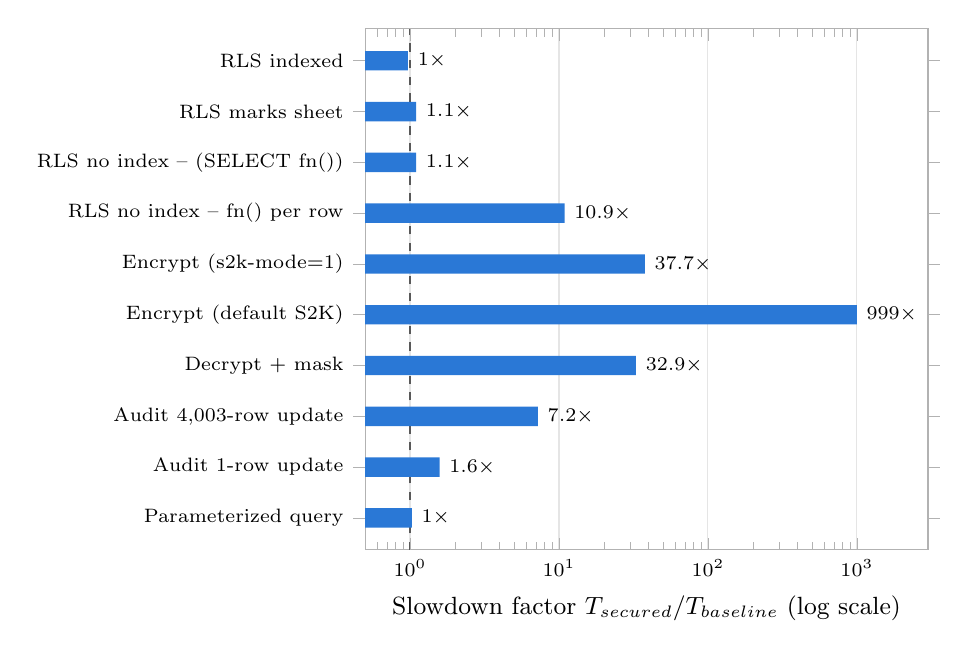
\begin{tikzpicture}
\begin{axis}[
    xbar, xmode=log, log origin=infty,
    width=0.72\textwidth, height=8.2cm,
    bar width=7pt,
    xmin=0.5, xmax=3000,
    xlabel={Slowdown factor $T_{secured}/T_{baseline}$ (log scale)},
    xlabel style={font=\small},
    symbolic y coords={Param,AuditOne,AuditBulk,Decrypt,EncDefault,EncS2K1,RLSNaive,RLSHoisted,RLSMarks,RLSIdx},
    ytick=data,
    yticklabels={Parameterized query, Audit 1-row update, Audit 4{,}003-row update, Decrypt + mask, Encrypt (default S2K), Encrypt (s2k-mode=1), RLS no index -- fn() per row, RLS no index -- (SELECT fn()), RLS marks sheet, RLS indexed},
    yticklabel style={font=\scriptsize},
    xticklabel style={font=\scriptsize},
    enlarge y limits=0.07,
    axis line style={gray!60},
    tick style={gray!60},
    xmajorgrids, major grid style={gray!20},
    nodes near coords={\pgfmathprintnumber[fixed,precision=1]{\pgfplotspointmeta}$\times$},
    nodes near coords style={font=\scriptsize, color=black, anchor=west},
    point meta=rawx,
    extra x ticks={1}, extra x tick labels={},
    extra x tick style={grid=major, major grid style={gray!70!black, dashed, thick}},
]
\addplot[fill=series1, draw=none] coordinates {
    (1.03,Param) (1.58,AuditOne) (7.23,AuditBulk) (32.9,Decrypt) (999,EncDefault)
    (37.7,EncS2K1) (10.9,RLSNaive) (1.10,RLSHoisted) (1.10,RLSMarks) (0.97,RLSIdx)
};
\end{axis}
\end{tikzpicture}
\caption{Relative cost of each control (1$\times$ = no overhead). Absolute costs are in Table~\ref{tab:perf}.}
\label{fig:perf}
\end{figure}

\subsubsection{Analysis and Impact on Usability}
\begin{itemize}
    \item \textbf{RLS is almost free when designed well.} With an index on the policy column and the helper wrapped as \texttt{(SELECT fn())}, faculty queries ran within noise of the unrestricted owner query, and the 3-table marks sheet was only 9.5\% slower (about 1\,ms). The \emph{same rule} written as \texttt{fn()} on an unindexed column was \textbf{11$\times$ slower}, because the function ran once for each of the 20,006 rows. Policy design, not RLS itself, decides the cost.
    \item \textbf{Encryption looks expensive in percent but is cheap in absolute terms.} Encrypting two columns adds about 21\,$\mu$s per registration, which no user can notice. Decryption costs about 7\,$\mu$s per value: a page listing 50 masked students adds under 1\,ms, while exporting all 20,000 masked records adds about 0.3\,s. The real danger was the \emph{default} key-stretching mode, which is \textbf{26$\times$ slower} (bulk registration of 20,000 students would take about 11\,s instead of 0.4\,s) and adds no security for a random 256-bit key.
    \item \textbf{Auditing has a visible cost only for bulk operations.} A single mark entry went from 0.12 to 0.18\,ms, which is imperceptible. Uploading 4,003 marks at once took 0.13\,s instead of 0.02\,s (about 28\,$\mu$s per row), still acceptable for an occasional bulk upload.
    \item \textbf{The SQL injection fix costs nothing.} Parameterized queries performed the same as string concatenation.
\end{itemize}

\subsection{Conflict Between Security, Usability and Performance}
\begin{table}[H]
    \centering
    \caption{Trade-off analysis and the resolution adopted}
    \label{tab:conflict}
    \footnotesize
    \setstretch{1.15}
    \begin{tabularx}{\textwidth}{|>{\raggedright\arraybackslash}p{2.3cm}|Y|Y|>{\raggedright\arraybackslash}p{2.1cm}|Y|}
        \hline
        \textbf{Control} & \textbf{Security gain} & \textbf{Usability cost} & \textbf{Measured performance cost} & \textbf{Resolution adopted} \\ \hline
        Per-user logins + RLS & Database enforces ``who sees what'' even if the application is buggy & More accounts to manage; harder connection pooling & $\approx$0--10\% & Group roles; scripted account creation; index policy columns \\ \hline
        Column privileges + masking & Faculty and accounts never see raw PII & Accounts can verify identity only by the last 4 digits & 7\,$\mu$s per masked value & Masked view for routine work; break-glass reveal for exceptions \\ \hline
        Column encryption & Stolen files and backups are useless & No \texttt{LIKE}, range search or sorting on PII & +21\,$\mu$s per insert & HMAC blind index for exact search; \texttt{s2k-mode=1} \\ \hline
        Break-glass reveal & Every disclosure is accountable; mass extraction blocked & Registrar must type a reason; 20 per day & Negligible & Limit is configurable; supervisors can raise it \\ \hline
        Audit triggers & Non-repudiation and forensics & Log grows; someone must review it & +58\% single row, 7$\times$ bulk & Store only changed columns; statement-level triggers for bulk loads (future) \\ \hline
        Parameterized queries & Removes SQL injection & Developer discipline needed & $\approx$0 & Enforced through code review \\ \hline
    \end{tabularx}
\end{table}

The main conclusion is that the conflict between security and performance is real, but it is concentrated in a few places (bulk audit and bulk decryption) that users rarely hit. Most of the cost found in testing came from \emph{design choices}, such as the default key stretching and unindexed policy functions, not from the security controls themselves. Measuring each control turned an assumed conflict into a set of specific, solvable engineering decisions.

\subsection{Proposed Solution Strategy}
\begin{table}[H]
    \centering
    \caption{Summary of the security architecture}
    \vspace{2mm}
    \setstretch{1.2}
    \begin{tabular}{|l|p{10cm}|}
        \hline
        \textbf{Strategy} & \textbf{Implementation Details} \\ \hline
        Threat Modelling & STRIDE analysis of 10 threats with $L \times I$ risk scoring; controls prioritised by risk. \\ \hline
        Access Control & Non-login owner, 5 group roles, personal logins, column-level grants, RLS policies, definer/invoker views. \\ \hline
        Injection Defence & Allow-list validation + parameterized queries; least privilege as the second layer. \\ \hline
        Encryption & AES-256 column encryption (\texttt{pgcrypto}), isolated key vault, HMAC blind index, TLS + SCRAM-SHA-256. \\ \hline
        Accountability & Change-capture triggers, audited break-glass PII access, append-only log readable only by auditors. \\ \hline
        Performance & Indexed policy columns, \texttt{(SELECT fn())} policies, \texttt{s2k-mode=1}, diff-only audit records. \\ \hline
    \end{tabular}
\end{table}

%% ------------------ Section 3: Program Outcome Mapping ------------------
%
%\section{Application of Program Outcomes and Sustainability Goals}
%As per the NBA SAR requirements for solving complex engineering problems incorporating sustainability, the following mapping demonstrates the technical and societal alignment of this report.
%
%\begin{table}[h!]
%    \centering
%    \renewcommand{\arraystretch}{1.4}
%    \setlength{\tabcolsep}{8pt}
%    \caption{Mapping of POs and Targeted Sustainability Goals}
%    \begin{tabular}{|c|p{8.5cm}|c|}
%        \hline
%        \textbf{PO No.} & \textbf{Relevance to Complex Engineering Problem Solving} & \textbf{Targeted SDG} \\
%        \hline
%        \textbf{PO1} & \textbf{Engineering Knowledge:} Applies access-control models, cryptography and DBMS internals to protect sensitive data. & SDG 16 \\
%        \hline
%        \textbf{PO2} & \textbf{Problem Analysis:} Builds a STRIDE threat model with quantified risk to identify the most critical threats. & SDG 16 \\
%        \hline
%        \textbf{PO3} & \textbf{Design/Development:} Designs RBAC, RLS, encryption and audit controls that satisfy the DPDP Act 2023. & SDG 16 \\
%        \hline
%        \textbf{PO4} & \textbf{Investigations:} Demonstrates SQL injection and measures the performance overhead of every control. & SDG 9 \\
%        \hline
%        \textbf{PO5} & \textbf{Tool Usage:} Uses PostgreSQL RLS, pgcrypto, Python/psycopg2 and benchmarking to engineer the solution. & SDG 9 \\
%        \hline
%        \textbf{PO11} & \textbf{Life-Long Learning:} Engages with evolving data-protection law and security practice beyond the syllabus. & SDG 4 \\
%        \hline
%    \end{tabular}
%\end{table}

% ------------------ Section 4: Sustainability ------------------

\section{Sustainability Integration}

\subsection{Efficient and Responsible Data Handling}
Security controls consume CPU time, storage and therefore energy, so they should be engineered as carefully as any other resource:
\begin{itemize}
    \item \textbf{Computation:} Choosing \texttt{s2k-mode=1} instead of the default removes about 96\% of the CPU work per encryption (20.97 vs.\ 555.90\,$\mu$s per row), with no loss of security for random keys. Writing RLS policies as \texttt{(SELECT fn())} avoids an 11$\times$ slowdown.
    \item \textbf{Storage:} The audit trigger stores only changed columns. A mark correction is logged as \texttt{\char`\{"internal": 38\char`\}} instead of the full row, which keeps the always-growing log small.
    \item \textbf{Data minimisation:} Staff see masked values by default, and plaintext is revealed only on demand. This follows the data-minimisation principle of the DPDP Act and reduces how much sensitive data is ever exposed.
\end{itemize}

\subsection{Impact on Society and Environment}
\begin{itemize}
    \item \textbf{Social:} Students' identity numbers and academic records are protected against theft, misuse and tampering. This upholds their right to privacy and their trust in the institution (\textbf{SDG 16}, \textbf{SDG 4}).
    \item \textbf{Economic:} Preventing a breach avoids regulatory penalties, legal costs and loss of reputation. Security built into the database also avoids repeated expensive fixes in each application.
    \item \textbf{Environmental:} Measuring overhead and removing wasteful cryptographic and query work lowers the energy needed to run the system securely.
\end{itemize}

% ------------------ Section 5: Conclusion ------------------

\section{Conclusion and Future Directions}

\subsection{Solution Summary}
A STRIDE threat model of a student information system identified ten threats, with SQL injection and mark tampering as the highest risks. The resulting design combines a non-login owner, five least-privilege group roles, column grants, row-level security and two kinds of views. Aadhaar and phone numbers are encrypted with AES-256 behind an isolated key vault, with a blind index for search, masked display and an audited, rate-limited break-glass reveal. Every change to sensitive tables is recorded in an append-only audit log that only auditors can read. An SQL injection that leaked the encryption keys and altered every mark through an over-privileged account was contained by least privilege and eliminated by parameterized queries. Measurements showed that well-designed RLS and parameterized queries are almost free. Encryption and auditing add only microseconds per row, so their cost matters only for bulk operations.

\subsection{Future Scope}
Future work includes moving the keys to an external \textbf{Key Management Service or Hardware Security Module} with envelope encryption and periodic key rotation. Statement-level auditing with the \textbf{pgAudit} extension, and \textbf{multi-factor authentication} for privileged users, are further steps. \textbf{Hash-chained audit records} would make tampering detectable even by a superuser. \textbf{Machine-learning anomaly detection} over the audit log could flag unusual access patterns, such as many reveals late at night. Finally, \textbf{statement-level triggers with transition tables} would reduce the bulk-audit overhead.

% ------------------ Section 6: References ------------------

\begin{thebibliography}{99}
    \bibitem{elmasri} R. Elmasri and S. B. Navathe, \textit{Fundamentals of Database Systems}, 7th Edition, Pearson Education, 2016 (Chapter 30: Database Security).
    \bibitem{silberschatz} A. Silberschatz, H. F. Korth and S. Sudarshan, \textit{Database System Concepts}, 7th Edition, McGraw-Hill Education, 2019.
    \bibitem{saltzer} J. H. Saltzer and M. D. Schroeder, ``The Protection of Information in Computer Systems,'' \textit{Proceedings of the IEEE}, Vol. 63, No. 9, pp. 1278--1308, 1975.
    \bibitem{shostack} A. Shostack, \textit{Threat Modeling: Designing for Security}, Wiley, 2014.
    \bibitem{halfond} W. G. J. Halfond, J. Viegas and A. Orso, ``A Classification of SQL-Injection Attacks and Countermeasures,'' \textit{Proc. IEEE International Symposium on Secure Software Engineering}, 2006.
    \bibitem{owasp} OWASP Foundation, \textit{SQL Injection Prevention Cheat Sheet} and \textit{OWASP Top 10:2021 -- A03 Injection}, \url{https://owasp.org}.
    \bibitem{pgdocs} The PostgreSQL Global Development Group, \textit{PostgreSQL 16 Documentation}: Row Security Policies, \texttt{CREATE VIEW}, and the \texttt{pgcrypto} module, \url{https://www.postgresql.org/docs/16/}.
    \bibitem{rfc4880} J. Callas et al., ``OpenPGP Message Format,'' RFC 4880, IETF, 2007.
    \bibitem{nist} E. Barker, \textit{Recommendation for Key Management: Part 1 -- General}, NIST Special Publication 800-57 Part 1 Rev. 5, 2020.
    \bibitem{dpdp} Government of India, \textit{The Digital Personal Data Protection Act, 2023} (No. 22 of 2023), and the Digital Personal Data Protection Rules, 2025.
\end{thebibliography}

\end{document}
